\section{Association:  making contact}
\subsection*{}

\begin{frame}
  \frametitle{How often do hard spheres touch?}

  \begin{block}{}
  A key input to Wertheim's TPT is the contact value of the
  correlation function of the hard-sphere fluid.
  \begin{itemize}
  \item Well known for a homogeneous fluid
  \item Two approximations for inhomogeneous systems
    \\ \hfill {\mycite{Yu and Wu}{J. Chem. Phys.}{2002}\tiny ;
    \mycite{Gross}{Surface Science}{2002}}
  \item Little justification, and no testing!
  \end{itemize}
  \end{block}
  \begin{center}
    
\includegraphics[height=3cm]{figs/HaglundChris}
    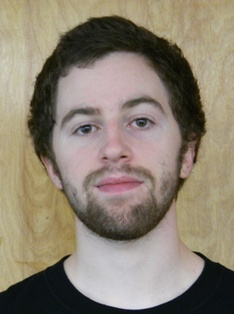
\includegraphics[height=3cm]{figs/KreitzbergPatrick}
    
\includegraphics[height=3cm]{figs/SchulteJeff}
  \end{center}
\end{frame}

\begin{frame}
  \frametitle{Finding the distribution function at contact $g_\sigma$}
  \vspace{-0.8em}
  \begin{center}
    \animategraphics[height=20em,autoplay]{.6}{anim/mc-gsigma-}{000}{30}\\
    \vspace{-2.0em}
    hard circles between two walls
  \end{center}
\end{frame}

\begin{frame}
  \frametitle{Monte Carlo:  spheres at a hard wall}
  \begin{columns}
    \begin{column}{0.5\columnwidth}
      \begin{center}
        low density\\
        \includegraphics[width=1.1\columnwidth]{figs/walls-mc-10}
      \end{center}
    \end{column}
    \begin{column}{0.5\columnwidth}
      \begin{center}
        high density\\
        \includegraphics[width=1.1\columnwidth]{figs/walls-mc-40}
      \end{center}
    \end{column}
  \end{columns}
\end{frame}

\begin{frame}
  \frametitle{Our theoretical approach}
  \begin{block}{Contact value theorem}
    Pressure on any hard surface is determined by the density of
    molecules in contact with it:
    \vspace{-1em}
    \[ p = n_{c}k_BT \]
    \vspace{-2em}
    \begin{itemize}
    \item We find pressure on spheres from a free energy derivative
      \vspace{-0.5em}
      \[p = \frac{1}{n(\rr)}\frac{1}{4\pi(2R)^2}\frac{\delta F_{HS}}{\delta R(\mathbf{r})}\]
    \item From the pressure, we know the density at contact
    \item From the density at contact, we find the correlation
      function
      \vspace{-0.5em}
      \[g_\sigma^A(\rr)
      = \frac{1}{n(\rr) n_A(\rr)}\frac{1}{ k_BT 4\pi (2R)^2} \frac{\delta
        F_{HS}}{\delta R(\mathbf{r})}\]
      \[
      n_A(\rr) = \int n(\rr')
      \frac{\delta(2R -|\rr-\rr'|)}{4\pi(2R)^2} d\rr' \label{eq:nA}
      \]
    \end{itemize}
  \end{block}
\end{frame}

\begin{frame}
  \frametitle{Results:  spheres at a hard wall}
  \begin{columns}
    \begin{column}{0.5\columnwidth}
      \begin{center}
        low density\\
        \includegraphics[width=1.1\columnwidth]{figs/walls-10}
      \end{center}
    \end{column}
    \begin{column}{0.5\columnwidth}
      \begin{center}
        high density\\
        \includegraphics[width=1.1\columnwidth]{figs/walls-40}
      \end{center}
    \end{column}
  \end{columns}
\end{frame}

\begin{frame}
  \frametitle{Results}
  \begin{center}
    Hard spheres at a hard wall, 10\% packing fraction\\
    \includegraphics[height=7cm]{figs/walls-10}
  \end{center}
\end{frame}

\begin{frame}
  \frametitle{Results}
  \begin{center}
    Hard spheres at a hard wall, 40\% packing fraction\\
    \includegraphics[height=7cm]{figs/walls-40}
  \end{center}
\end{frame}

\begin{frame}
  \frametitle{\conclude}
  \begin{center}
    \includegraphics[height=4cm]{figs/walls-10}
    \includegraphics[height=4cm]{figs/walls-40}
  \end{center}
  \begin{itemize}
  \item Derived and tested an accurate functional for the correlation
    function at contact for hard spheres
  \item Reasonably efficient: scales like the hard sphere free energy
  \end{itemize}
\end{frame}
